% Created 2022-10-20 Thu 14:06
% Intended LaTeX compiler: pdflatex
\documentclass[11pt,onecolumn]{scrartcl}
\usepackage[utf8]{inputenc}
\usepackage[T1]{fontenc}
\usepackage{graphicx}
\usepackage{longtable}
\usepackage{wrapfig}
\usepackage{rotating}
\usepackage[normalem]{ulem}
\usepackage{amsmath}
\usepackage{amssymb}
\usepackage{capt-of}
\usepackage{hyperref}
\usepackage{xcolor}
\usepackage{listings}
\definecolor{base03}{HTML}{002b36}
\definecolor{base02}{HTML}{073642}
\definecolor{base01}{HTML}{586e75}
\definecolor{base00}{HTML}{657b83}
\definecolor{base0}{HTML}{839496}
\definecolor{base1}{HTML}{93a1a1}
\definecolor{base2}{HTML}{eee8d5}
\definecolor{base3}{HTML}{fdf6e3}
\definecolor{yellow}{HTML}{b58900}
\definecolor{orange}{HTML}{cb4b16}
\definecolor{red}{HTML}{dc322f}
\definecolor{magenta}{HTML}{d33682}
\definecolor{violet}{HTML}{6c71c4}
\definecolor{blue}{HTML}{268bd2}
\definecolor{cyan}{HTML}{2aa198}
\definecolor{green}{HTML}{859900}
\lstset{
language=R,
linewidth=0.95\textwidth,
xleftmargin=0.05\textwidth,
basicstyle=\small\ttfamily\color{base02},
backgroundcolor=\color{base3},
showspaces=false,
showstringspaces=false,
showtabs=false,
frame=single,
frameround=tttt,
float=p,
rulecolor=\color{base03},
tabsize=2,
captionpos=b,
breaklines=true,
breakatwhitespace=false,
keywordstyle=\color{base02},
commentstyle=\color{base02},
stringstyle=\color{cyan}
}
\usepackage{fancyvrb}
\usepackage[
figurename=Figure,
font={sf,small},
format=plain,
labelfont=bf,
width=0.7\textwidth
]{caption}
\setcounter{secnumdepth}{2}
\author{Alexander E. Zarebski}
\date{\today}
\title{Git, GitHub and Reproducible Research}
\hypersetup{
 pdfauthor={Alexander E. Zarebski},
 pdftitle={Git, GitHub and Reproducible Research},
 pdfkeywords={},
 pdfsubject={},
 pdfcreator={Emacs 28.2 (Org mode 9.5.5)},
 pdflang={English}}
\begin{document}

\maketitle
\setcounter{tocdepth}{2}
\tableofcontents


\section{Introduction}
\label{sec:org165ff97}

Welcome to \emph{Git, GitHub and Reproducible Research}! In this tutorial we will
look at ways git and GitHub can help you with computational research, including
how make it more reproducible. You will learn the fundamentals of git and gain
practical experience in the use of GitHub. For those interested in learning more
about version control, there is also a list of \hyperref[sec:orgb20342f]{additional resources} and some
\hyperref[sec:org2dd58c7]{homework problems} at the end to test your understanding.

Please read through the \hyperref[sec:org5363665]{background material} first then follow along with the \hyperref[sec:org9c3a0e3]{worked example}. You do not need any special software installed (everything is
done in the browser), however the worked example does make use of R and ggplot2.
Installing \href{https://www.rstudio.com/}{RStudio} is probably the easiest way to utilise these software. If you
find an error in this document, or would like to suggest an improvement, please
make a note of this in the \href{https://github.com/aezarebski/github-tutorial/issues/new/choose}{issue tracker} on GitHub.

\section{Disclaimer}
\label{sec:org7c8be1f}

These materials makes use of proprietary products and a simplified workflow in
order to emphasise the main concepts and to save on installation and
configuration time. Some references will be given at the end to direct you to
free and open source solutions and more sustainable workflows; the core ideas
are the same though, so understanding the material given here should make it
easier to migrate to more advanced methods in the future should the need for
them arise.

\section{Background material}
\label{sec:org5363665}

This section provides some context for why you might care about git, GitHub and
reproducible research. This document only provides the absolute basics of these
topics but should get you started with them and help direct further learning.

\subsection{Version control}
\label{sec:orgc42377c}

\emph{Version control} refers to systems which help to manage the writing and
maintenance of things such as software, documents, and websites. These systems
were developed to manage large software projects but are useful at many levels.
For example, version control can help you avoid the following situation:
\texttt{my-analysis.R}, \texttt{my-analysis-final.R}, \texttt{my-analysis-final-again.R}, and so on.
Try coming back to that 3 months later when a reviewer asks you to re-run
something with a slight modification!

\subsubsection*{Reproducible research and Open research}
\label{sec:orge5424b7}

In addition to helping \textbf{you} with organising your files, a version control
system and it's associated tooling can also help the scientific community by
helping to make your research reproducible and open.

For your computational research to be considered \emph{reproducible,} it needs to be
described in such a way that others can replicate your results. For it to be
\emph{open}, the materials (code, data and sufficient documentation) need to be
available for others. Simply dumping all of your code into something like GitHub
is not sufficient for your research to be considered reproducible.

\subsection{Git}
\label{sec:orga0c6e09}

Created in 2005 by Linus Torvalds\footnote{Legend has it, he named git after himself.} to help with the development of the
Linux kernel, git has become a fundamental tool for software development. In the
2021 Stackoverflow Developer Survey over \(90\%\) of respondents used git; it is
nearly synonymous with version control. If you intend to collaborate in the
writing of substantial amounts of code, taking the time to learn how to use git
is a good idea, at which point you may want to switch to a \hyperref[sec:org199274b]{GUI interface} too.

Working with git will be much easier if you get familiar with some of the
terminology first. Unless you are familiar with git already, you should at least
skim these before continuing.

\subsubsection*{Repository}
\label{sec:org195bba2}

A \emph{repository} is a directory containing your files and the history of all the
edits (see \hyperref[sec:org6c2793a]{commit}) made to these files. You can have a repository that only
lives on your machine, but they are often shared on a platform such as GitHub.

\subsubsection*{Commit}
\label{sec:org6c2793a}

An edit to a file that you have recorded as part of the history of edits is
called a \emph{commit}. It is both a noun and a verb, you commit an edit and the
\hyperref[sec:org195bba2]{repository} contains all of your commits. This can be thought of as a stronger
version of saving a file. Each commit gets a unique identifier (called a
\emph{hash}). Sometimes we use "commit" to refer to the state of all the code after
an edit.

\subsubsection*{Clone}
\label{sec:orgd9fcb88}

When you make a copy of a \hyperref[sec:org195bba2]{repository} you are \emph{cloning} that repository. The
resulting copy is referred to as a \emph{clone}. Typically this will mean you have
downloaded a copy from a platform such as GitHub.

\subsubsection*{Pull}
\label{sec:org220a7ce}

Suppose you \hyperref[sec:orgd9fcb88]{cloned} a repository a while ago and you want to get a copy of all
the \hyperref[sec:org6c2793a]{commits} that have been made to the original repository since then. To get
these commits you \emph{pull} them, which is a fancy way of saying updating your
files. This is sometimes referred to as \emph{fetching}. There are some subtle
differences that you probably won't ever need.

\subsubsection*{Push}
\label{sec:org0f7128f}

If you have \hyperref[sec:org6c2793a]{committed} some changes to your \hyperref[sec:orgd9fcb88]{clone} of a \hyperref[sec:org195bba2]{repository} and want the
original repository to have these changes made, you \emph{push} these changes. This
is a fancy way of saying use your edits to update the original files.

\subsubsection*{Branch}
\label{sec:org43a575d}

A \emph{branch} is similar to a \hyperref[sec:orgd9fcb88]{clone} in that it is a copy of a \hyperref[sec:org195bba2]{repository}. This
provides a more sophisticated way for people to work on their own version of
code, without messing up the main copy. This is not particularly important
unless you are collaborating with others on a project.

\subsubsection*{Merge}
\label{sec:org8f2ea49}

If someone has made some useful changes on their \hyperref[sec:org43a575d]{branch} the owner of the
repository may decide to include their commits in the main copy. This process of
including the changes on someone's branch is called \emph{merging} the changes.

\subsubsection*{Fork}
\label{sec:orgab389f5}

When you make a copy of a repository that sits on your GitHub account. This is
similar to, (but distinct from) \hyperref[sec:orgd9fcb88]{cloning} and making a \hyperref[sec:org43a575d]{branch}. Forking a
repository is an important part of contributing code to other peoples' projects
when using GitHub, however the details of this are beyond the scope of this
tutorial.

\subsubsection*{Pull request (a.k.a. PR)}
\label{sec:org9ad35a4}

A pull request is a way to request that the owner of a repository accepts the
changes you are proposing. As with \hyperref[sec:orgab389f5]{forking}, the details are of this are beyond
the scope of this tutorial.

\subsubsection*{Client}
\label{sec:org199274b}

A \emph{git client} is a program that "simplifies" the use of git. We will only use
the GitHub website in this tutorial because it handles most of this for us and
avoids any complicated installation. If you are going to be making substantial
use of git, I would recommend getting a client and learning how to use it.
\href{https://desktop.github.com/}{GitHub Desktop} and \href{https://www.sourcetreeapp.com/}{Sourcetree} are both free options developed by major companies
so should be very friendly\footnote{I use \href{https://magit.vc/}{magit}, which is nice if you already use emacs, but otherwise may be a bit weird.}.

If you are already using RStudio, you might also be interested in the features
it provides for version control. There is a \href{https://resources.github.com/github-and-rstudio/}{tutorial on using RStudio as a
GitHub client}, but it requires some command line experience and for both RStudio
and git to be installed on your machine.

\subsection{GitHub}
\label{sec:org797c4bb}

\subsubsection*{What is GitHub?}
\label{sec:org01ee6b9}

GitHub, Inc. is a subsidiary of Microsoft. Their website provides freemium
hosting of git repositories. In addition to hosting the repositories, it offers
additional tools to assist with software development. We will use GitHub in this
tutorial to avoid you needing to install anything on your machine. If you are
going to use git extensively, it would be wise to learn how to do this from the
command line or some other \hyperref[sec:org199274b]{program}.

\subsubsection*{Setting up a GitHub account}
\label{sec:org48508de}

To register an account you will need an email address that can be used for
verification. A Gmail account makes this particularly easy.

\begin{enumerate}
\item Visit \url{https://github.com/} and click \textbf{Sign Up}.
\item Fill in the forms to create an account.
\item Verify that account by entering the access code GitHub sends to the email
address you registered with.
\item Verify that you can summon the \textbf{Command Palette} with \texttt{crtl k} for Windows
and Linux and \texttt{command k} on a mac.
\item The appearance and accessibility settings can be reached by searching for
them in the command palette.
\end{enumerate}

\subsection{Zenodo}
\label{sec:org74e3e7c}

Zenodo is an open access archive operated by CERN which allows researchers to
archive research materials with a DOI which makes them easier to cite. This is a
more permanent form of storage than GitHub. It is easy to archive a particular
commit of a repository which is good practice if you want to refer to a
particular version of some code in a paper.

\section{Worked example}
\label{sec:org9c3a0e3}

Now that we have an understanding of version control and its associated tooling,
we can see an example of how this enables us to do more reproducible research.
Suppose you wanted to ensure that the analysis leading to Figure
\ref{fig:demo-result-1} was reproducible. In this worked example we will work through
the process of setting up a repository and uploading the relevant files. A copy
of the resulting repository is available \href{https://github.com/aezarebski/git-usage}{here}.

\begin{figure}[htbp]
\centering
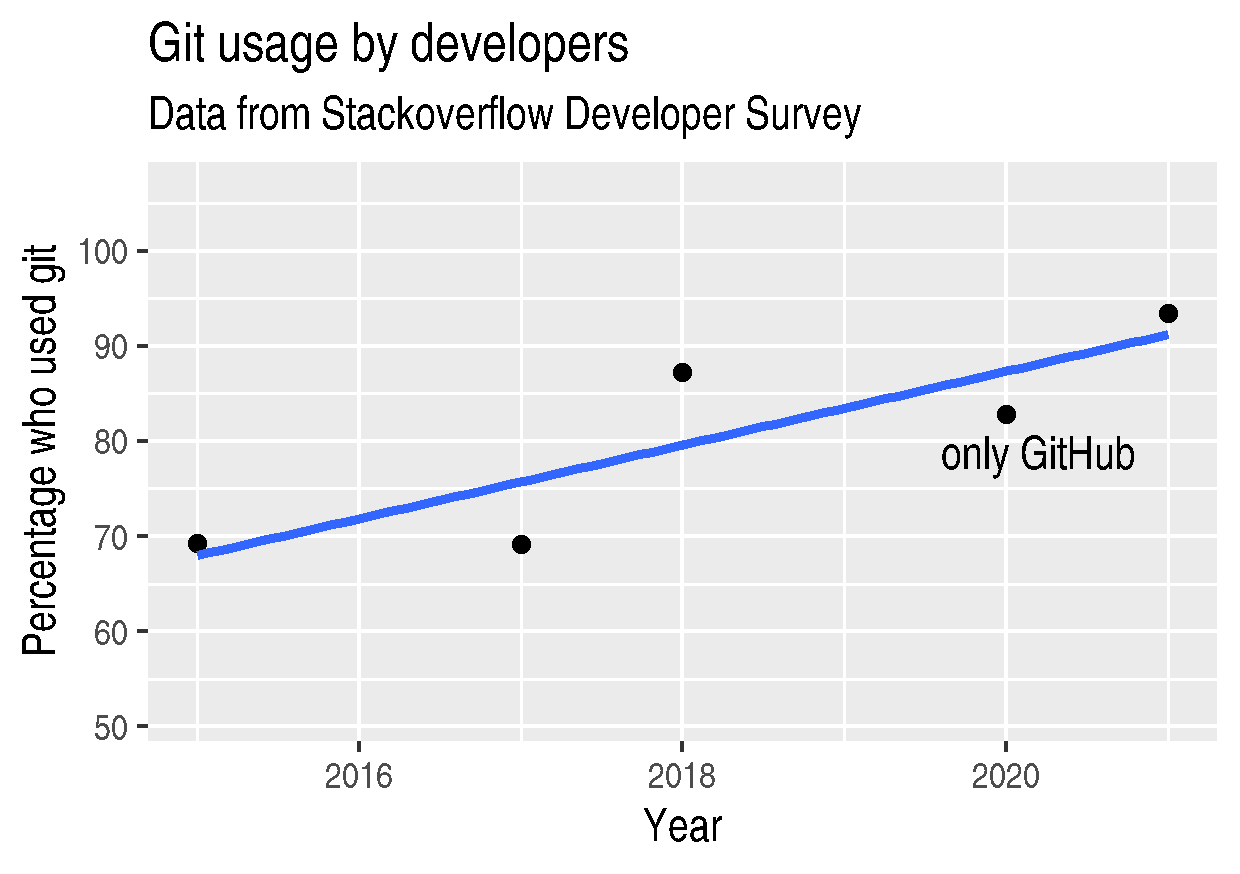
\includegraphics[width=8cm]{./git-usage-1.png}
\caption{\label{fig:demo-result-1}The percentage of developers who use git has increased since 2015. Data from the Stackoverflow Developer Survey is shown as black points and a least squares regression is shown as a blue line, the trend is not significant at \(95\%\).}
\end{figure}

We will start by looking at the \hyperref[sec:orga4e5ff3]{code and data} used in this analysis, then
consider how one might \hyperref[sec:org0958a85]{organise the files}. Once we have the code in a sensible
state we can \hyperref[sec:org56a7d86]{put it in a GitHub repository} and add some finishing touches such
as a \hyperref[sec:org2a4f957]{license}, some \hyperref[sec:org49947a3]{documentation}, and some additional \hyperref[sec:org3d977e1]{information about package
versions}. We then consider the situation in which \hyperref[sec:orga8bc06b]{changes} need to be made by a
collaborator.

\subsection{Code and data}
\label{sec:orga4e5ff3}

Start by making a new directory called \texttt{git-usage} which will hold all our
files. The data and the code that generated this figure are included below. This
data should be saved in a called \texttt{stackoverflow-git-data.csv}.

\begin{Verbatim}[frame=single,framerule=0.5mm,framesep=2mm,label=Git Usage,xleftmargin=5cm,xrightmargin=5cm]
year,percentage
2015,69.3
2017,69.2
2018,87.2
2020,82.8
2021,93.43
\end{Verbatim}

We then need a script to carry out the analysis. Save the following code in a
file called \texttt{make-plot.R}

\lstset{language=r,label= ,caption= ,captionpos=b,numbers=none}
\begin{lstlisting}
library(ggplot2)

sods_data <- read.csv("stackoverflow-git-data.csv")

g <- ggplot(
  data = sods_data,
  mapping = aes(x = year, y = percentage)) +
  geom_point() +
  geom_smooth(method = "lm") +
  geom_text(
    aes(x = 2020, y = 82.8, label = "only GitHub"),
    nudge_x = 0.2,
    nudge_y = -4) +
  labs(
    x = "Year",
    y = "Percentage who used git",
    title = "Git usage has increased",
    subtitle = "Data from Stackoverflow Developer Survey")

ggsave(filename = "git-usage.png",
       plot = g,
       height = 7.4,
       width = 10.5,
       units = "cm")

sink(file = "regression-summary.txt")
summary(lm(percentage ~ year, data = sods_data))
sink()
\end{lstlisting}

Once we have run the \texttt{make-plot.R} script, the directory should contain four files
and have a structure like the following.

\begin{Verbatim}[frame=single,framerule=0.5mm,framesep=2mm,label=Directory contents,xleftmargin=3cm,xrightmargin=3cm]
  git-usage
  +-- git-usage.png
  +-- make-plot.R
  +-- regression-summary.txt
  +-- stackoverflow-git-data.csv
\end{Verbatim}

In the next section we will go through cleaning this up so it is easier for
people (including yourself in the future) to make sense of this.

\subsection{Organising the data and code}
\label{sec:org0958a85}

As a first step we will use directories to impose a sensible structure to our
files. Organising files in this way is useful as it makes it far easier for
someone to understand what each file is needed for. Follow the following steps
(starting from within \texttt{git-usage},) to organise your code more appropriately:

\begin{enumerate}
\item Make a directory called \texttt{src} and move \texttt{make-plot.R} there.
\item Make a directory called \texttt{data} and move \texttt{stackoverflow-git-data.csv} there.
\item Make a directory called \texttt{out} which we will write results to.
\item Fix the call to \texttt{read.csv} in \texttt{make-plot.R} so it can find the CSV since it
now lives in the \texttt{data} directory.
\item Fix the calls to \texttt{ggsave} and \texttt{sink} so they write their output to the \texttt{out}
directory.
\end{enumerate}

Once you have done this, the R script should look like the following.

\lstset{language=r,label= ,caption= ,captionpos=b,numbers=none}
\begin{lstlisting}
sods_data <- read.csv("data/stackoverflow-git-data.csv")

...

ggsave(filename = "out/git-usage.png",
       plot = g,
       height = 7.4,
       width = 10.5,
       units = "cm")

sink(file = "out/regression-summary.txt")
summary(lm(percentage ~ year, data = sods_data))
sink()
\end{lstlisting}

Once you have run the code (with \texttt{git-usage} as your working directory), the
directory structure should look like the following. Note how the output files
now appear in the \texttt{out} directory. If you are running the script from an R REPL,
remember you can use \texttt{setwd} to specify the working directory.

\begin{Verbatim}[frame=single,framerule=0.5mm,framesep=2mm,label=Git Usage,xleftmargin=3cm,xrightmargin=3cm]
git-usage
+-- data
|   +-- stackoverflow-git-data.csv
+-- out
|   +-- git-usage.png
|   +-- regression-summary.txt
+-- src
    +-- make-plot.R
\end{Verbatim}

\subsection{Uploading to GitHub}
\label{sec:org56a7d86}

Now that our code is in a reasonable state, we can upload it to GitHub. If you
do not already have a GitHub account, please follow the instructions \hyperref[sec:org48508de]{above},
which describe how to make one. Once you have a GitHub account, you can follow
the following steps to upload these files:

\begin{enumerate}
\item Visit \url{https://github.com/} and create a new \hyperref[sec:org195bba2]{repository} by clicking \textbf{New}, you
will need to pick a name for the repository (I called mine \texttt{git-usage}.) The
default settings provided by GitHub are fine. Click \textbf{Create repository}.
\item We now need to \hyperref[sec:org6c2793a]{commit} our files and \hyperref[sec:org0f7128f]{push} them to the remote repository.
However, since we are doing this through GitHub, it is all combined into a
single step. Click \textbf{Add file} and then \textbf{creating a new file} to start the
process of adding the \texttt{src/make-plot.R} file.
\begin{enumerate}
\item Ensure the name of the file is \texttt{git-usage/src/make-plot.R} (be careful
that you have the \emph{path} with the \texttt{\textbackslash{}} correct.)
\item Copy-and-paste the code in \texttt{make-plot.R} into the text box provided.
\item Click \textbf{Commit new file} button.
\end{enumerate}
If you are struggling to make a new directory in GitHub, see the next
section.
\item Repeat this process with \texttt{data/stackoverflow-git-data.csv} and the output TXT
file. In the case of the PNG image, \texttt{git-usage.png}, you will need to use
\textbf{Upload file} instead of \textbf{Create new file}.
\end{enumerate}

\subsection{Making directories via GitHub}
\label{sec:org1dfcf8f}

You cannot add an empty directory to a GitHub directory. If you want a new
directory to be added, you need to commit a file to it. One convention for this
is to make an empty file in the desired directory (often this will be a file
called \texttt{.gitkeep}).

\subsection{Adding a license}
\label{sec:org2a4f957}

A license specifies what people can do with your code. If you aren't sure what
license suits your needs, you might find \url{https://choosealicense.com/} has some
helpful information. Most of the time, I will opt for the MIT license.

There are two ways you might add a license. The manual method is to copy and
paste the license text into a file called \texttt{LICENSE} to your repository, filling in
\texttt{[year]} and \texttt{[fullname]} as appropriate. Alternatively, you can \textbf{Add file} and \textbf{Create
new file} and specify that the file will be called "LICENSE" and it will offer
you some templates to choose from. It will auto-fill the details of your name
and the year.

\subsection{Adding a README}
\label{sec:org49947a3}

When you encounter a repository online it can be difficult to understand what
its purpose is and how to use it. "README" is the name given to a file that
contains this sort of information. Typically these will be written in markdown
(similar to RMarkdown). Add a file called \texttt{README.md} to your repository with text
similar to the following.

\lstset{language=sh,label= ,caption= ,captionpos=b,numbers=none}
\begin{lstlisting}
This repository contains an analysis of git usage through time.

To run this analysis use the following command:

```
Rscript src/make-plot.R
```

The input data is in `data` and the results are in `out`.
\end{lstlisting}

\subsection{Recording the session information}
\label{sec:org3d977e1}

Software gets updated, and sometimes these updates cause things to break. Where
possible, it is very good practise to include details of the versions of
software you have used. When working with R the \texttt{sessionInfo} command makes this
simple. Try adding the following to the end of the \texttt{make-plot.R} script.

\lstset{language=r,label= ,caption= ,captionpos=b,numbers=none}
\begin{lstlisting}
sink(file = "out/package-versions.txt")
sessionInfo()
sink()
\end{lstlisting}

The next time that you run this script, it will write a description of the
version of R you used and the versions of all the loaded packages to the file
\texttt{out/package-versions.txt}. Try running the script again to make sure this
additional file was generated and contains something similar to the following.

\begin{Verbatim}[frame=single,framerule=0.5mm,framesep=2mm,label=Session information,xleftmargin=5mm,xrightmargin=5mm,fontsize=\small]
R version 4.1.2 (2021-11-01)
Platform: x86_64-pc-linux-gnu (64-bit)
Running under: Ubuntu 20.04.3 LTS

Matrix products: default
BLAS:   /usr/local/lib/R/lib/libRblas.so
LAPACK: /usr/local/lib/R/lib/libRlapack.so

locale:
 [1] LC_CTYPE=en_GB.UTF-8       LC_NUMERIC=C
 [3] LC_TIME=en_GB.UTF-8        LC_COLLATE=en_GB.UTF-8
 [5] LC_MONETARY=en_GB.UTF-8    LC_MESSAGES=en_GB.UTF-8
 [7] LC_PAPER=en_GB.UTF-8       LC_NAME=C
 [9] LC_ADDRESS=C               LC_TELEPHONE=C
[11] LC_MEASUREMENT=en_GB.UTF-8 LC_IDENTIFICATION=C

attached base packages:
[1] stats     graphics  grDevices utils     datasets  methods   base

other attached packages:
[1] ggplot2_3.3.5

loaded via a namespace (and not attached):
 [1] magrittr_2.0.1   splines_4.1.2    tidyselect_1.1.1 munsell_0.5.0
 [5] colorspace_2.0-2 lattice_0.20-45  R6_2.5.1         rlang_0.4.12
 [9] fansi_0.5.0      dplyr_1.0.7      tools_4.1.2      grid_4.1.2
[13] gtable_0.3.0     nlme_3.1-153     mgcv_1.8-38      utf8_1.2.2
[17] withr_2.4.3      ellipsis_0.3.2   digest_0.6.29    tibble_3.1.6
[21] lifecycle_1.0.1  crayon_1.4.2     Matrix_1.3-4     farver_2.1.0
[25] purrr_0.3.4      vctrs_0.3.8      glue_1.6.0       labeling_0.4.2
[29] compiler_4.1.2   pillar_1.6.4     generics_0.1.1   scales_1.1.1
[33] pkgconfig_2.0.3
\end{Verbatim}

Once you are happy that this has worked, we need to commit these changes. First
by editing the script, and second, add the \texttt{package-versions.txt} file.

\subsection{Branching and merging}
\label{sec:orga8bc06b}

Suppose that after doing all of this one of your collaborators wants to adjust
the figure. We will now go through the steps involved with doing this using
branches.

\subsubsection*{Branching to make changes}
\label{sec:org74b4d61}

Figure \ref{fig:demo-result-2} is a modification of Figure \ref{fig:demo-result-1} with the
desired changes.

\begin{figure}[htbp]
\centering
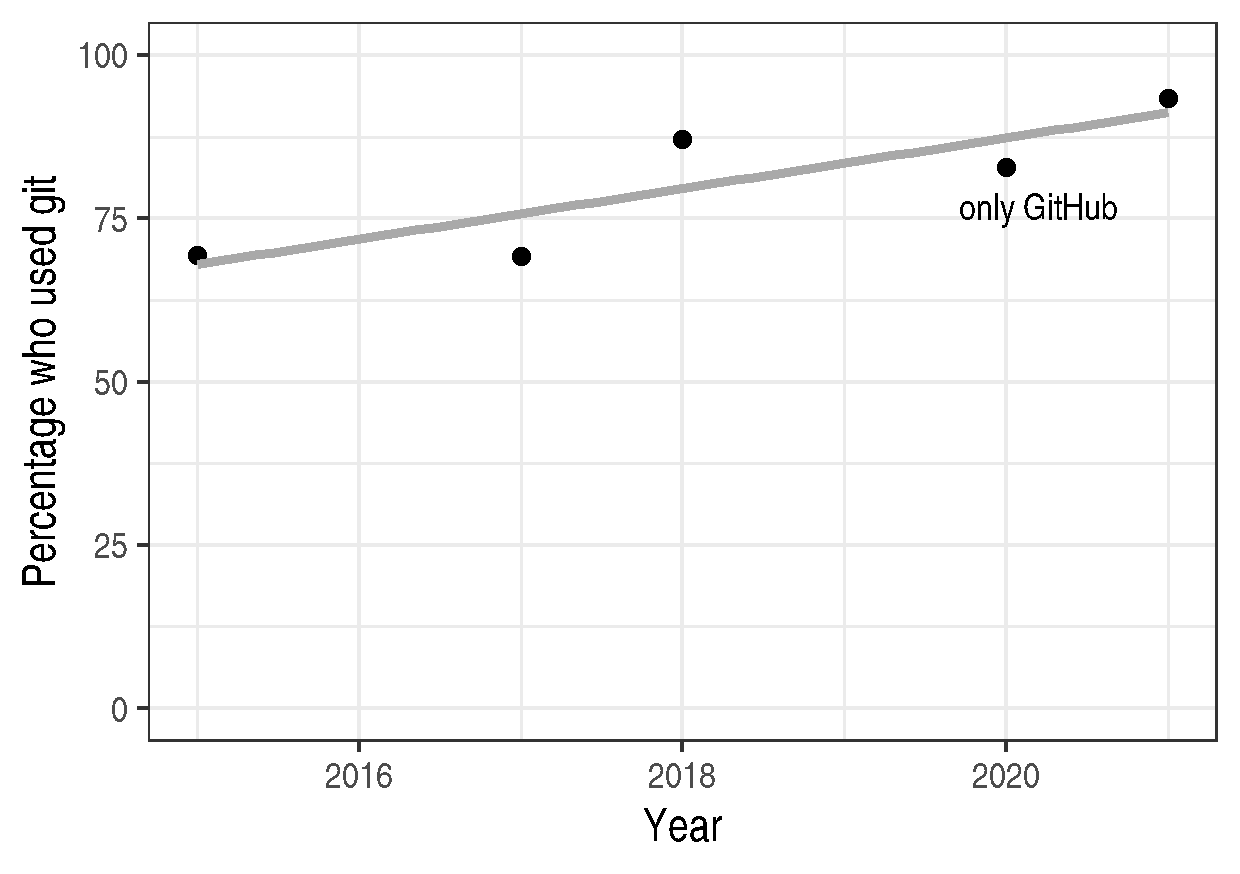
\includegraphics[width=8cm]{./git-usage-2.png}
\caption{\label{fig:demo-result-2}The percentage of developers who use git has increased since 2015. Data from the Stackoverflow Developer Survey is shown as black points and a least squares regression is shown as a grey line, the trend is not significant at \(95\%\).}
\end{figure}

To avoid making changes to the main copy of the code we will work on a \hyperref[sec:org43a575d]{branch},
and then when we are happy with the changes we will \hyperref[sec:org8f2ea49]{merge} them. To start with,
create a new branch by clicking on the drop-down menu labelled "main" as shown
in Figure \ref{fig:create-new-branch}. I called it "edit-plot", but you can use
anything other than "main" (because that is the default branch name used by
GitHub).

\begin{figure}[htbp]
\centering
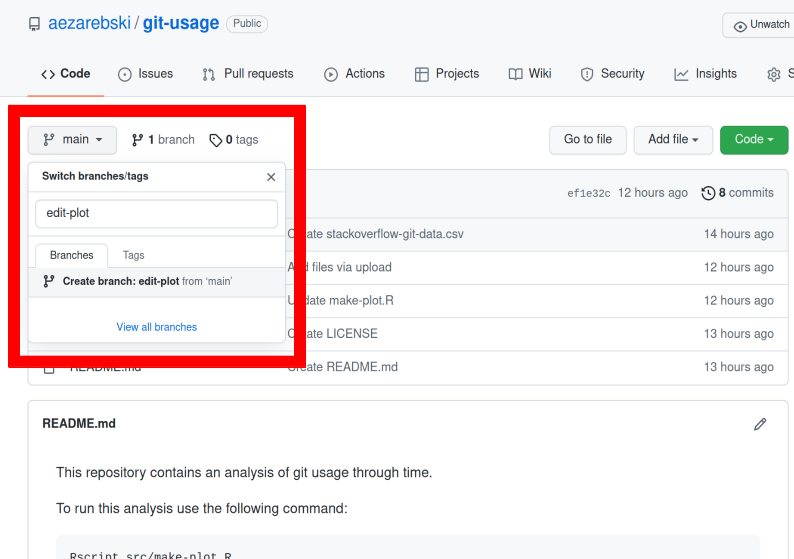
\includegraphics[width=8cm]{./create-new-branch.png}
\caption{\label{fig:create-new-branch}Create a new branch using the drop-down menu.}
\end{figure}

\subsubsection*{Make desired edits to the code and output}
\label{sec:org8504497}

\uline{Making sure that you are on your branch} --- if you're not sure, click on the
\textbf{branch} button to double check --- edit the \texttt{make-plot.R} script so that it has the
following

\lstset{language=r,label= ,caption= ,captionpos=b,numbers=none}
\begin{lstlisting}
g <- ggplot(
  data = sods_data,
  mapping = aes(x = year, y = percentage)) +
  geom_point() +
  geom_smooth(method = "lm", colour = "darkgrey") +
  geom_text(
    aes(x = 2020, y = 82.8, label = "only GitHub"),
    size = 3,
    nudge_x = 0.2,
    nudge_y = -6) +
  labs(
    x = "Year",
    y = "Percentage who used git") +
  ylim(c(0,100)) +
  theme_bw()
\end{lstlisting}

Once you have made the changes and re-run that script the figure in
\texttt{git-usage.png} will have changed --- it should look like Figure \ref{fig:demo-result-2}
now. Ordinarily, you would update the figure in the same way that you update
code, by committing the changes. However, this is tricky to do via the GitHub
website for image files, so instead, delete the file and upload the modified
one. At this point it might be interesting to move between the \texttt{main} branch and
your new branch to see how the files change between the two.

One motivation for branches is that you can make exploratory changes without
risking messing up your code on the main branch. If you have a collaborator that
wanted to try something, they could do so on a separate branch and then, if you
like their edits, you can \hyperref[sec:org8f2ea49]{merge} them into \texttt{main} as we are about to do now.

\subsubsection*{Merge the changes}
\label{sec:org12e8180}

To \hyperref[sec:org8f2ea49]{merge} your changes via the website, go back to the main page of the
repository and you should see a new button, like the one shown in Figure
\ref{fig:pull-request}, inviting you to compare the changes on this branch, i.e., to
inspect if you consider this work worthy of inclusion.

\begin{figure}[htbp]
\centering
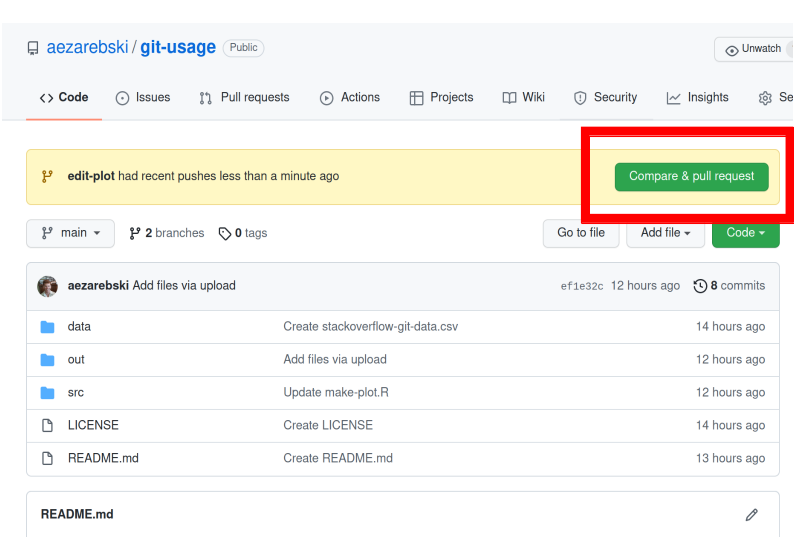
\includegraphics[width=8cm]{./pull-request.png}
\caption{\label{fig:pull-request}A button appears to invite you to compare branches.}
\end{figure}

Inspect the differences between the branches and if you are happy with them
create a pull request by clicking the button as shown in Figure
\ref{fig:create-pull-request}.

\begin{figure}[htbp]
\centering
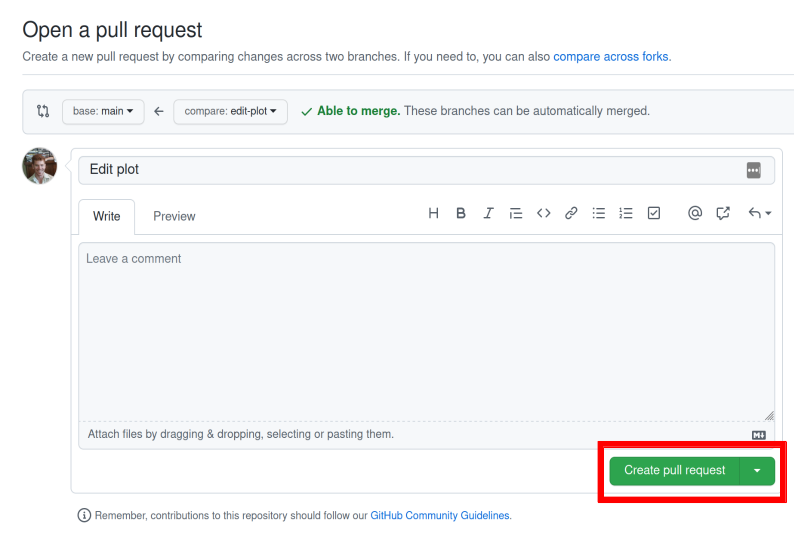
\includegraphics[width=8cm]{./create-pull-request.png}
\caption{\label{fig:create-pull-request}If you are happy with the content of a branch, you can create a pull request.}
\end{figure}

Once you have created the pull request, the next step is to \hyperref[sec:org8f2ea49]{merge} that branch
into the \texttt{main} branch. To do this you just need to click the button shown in
Figure \ref{fig:merge-pull-request}.

\begin{figure}[htbp]
\centering
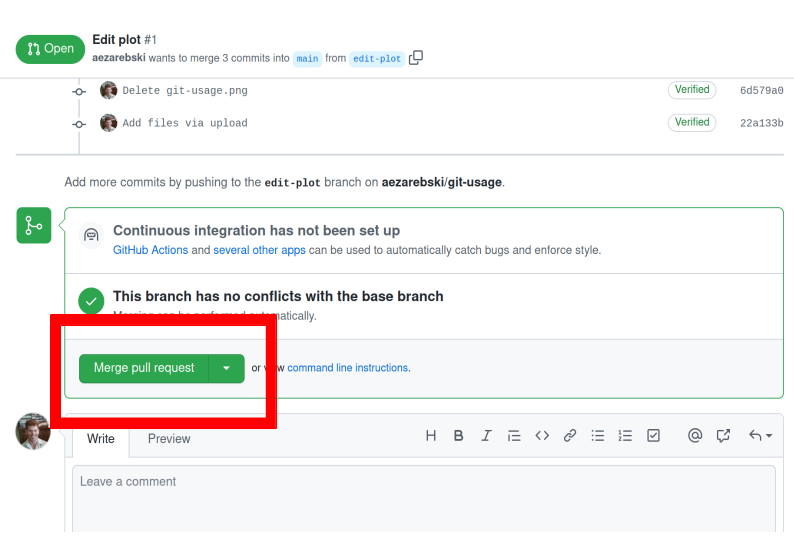
\includegraphics[width=8cm]{./merge-pull-request.png}
\caption{\label{fig:merge-pull-request}If you accept a pull request you can merge the changes with the Merge pull request button.}
\end{figure}

Once a branch has been merged it will hang around until you delete it. Since
having old branches around can lead to confusion, it is sensible to delete them
afterwards. As shown in Figure \ref{fig:delete-branch} there is a button to achieve
this.

\begin{figure}[htbp]
\centering
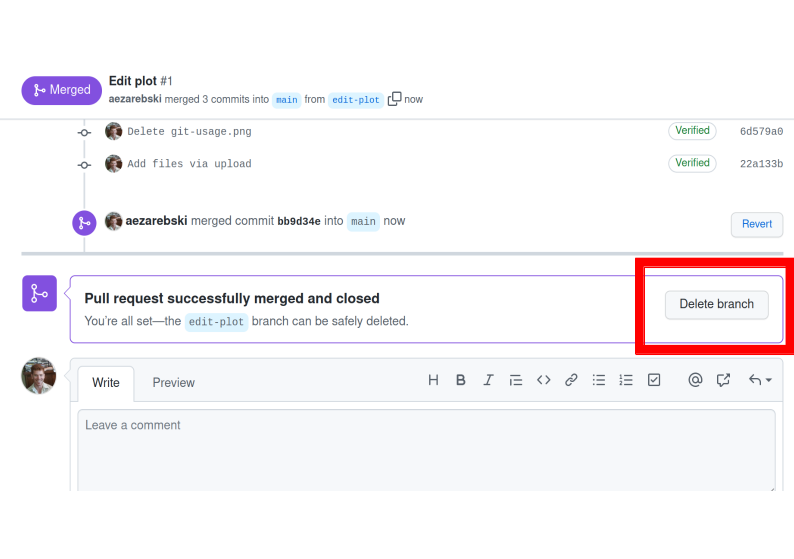
\includegraphics[width=8cm]{./delete-branch.png}
\caption{\label{fig:delete-branch}Deleting a branch after it has been merged keeps the repository tidy.}
\end{figure}

At this point you should only have a single branch left and it should have the
modifications to the figure. Congratulations on a reproducible analysis!

\section{Next steps and alternative solutions}
\label{sec:orgb20342f}

\subsection{Help! I just want to download the files}
\label{sec:orgac9079d}

If you want to download the files from GitHub and do not want any of the
associated git functionality, you can download a ZIP file that contains the
contents of a repository. Figure \ref{fig:download-zip-file} shows the menu for
downloading a ZIP file containing the contents of a repository. If you want to
use any of git's features though you should \hyperref[sec:orgd9fcb88]{clone} the repository instead.

\begin{figure}[htbp]
\centering
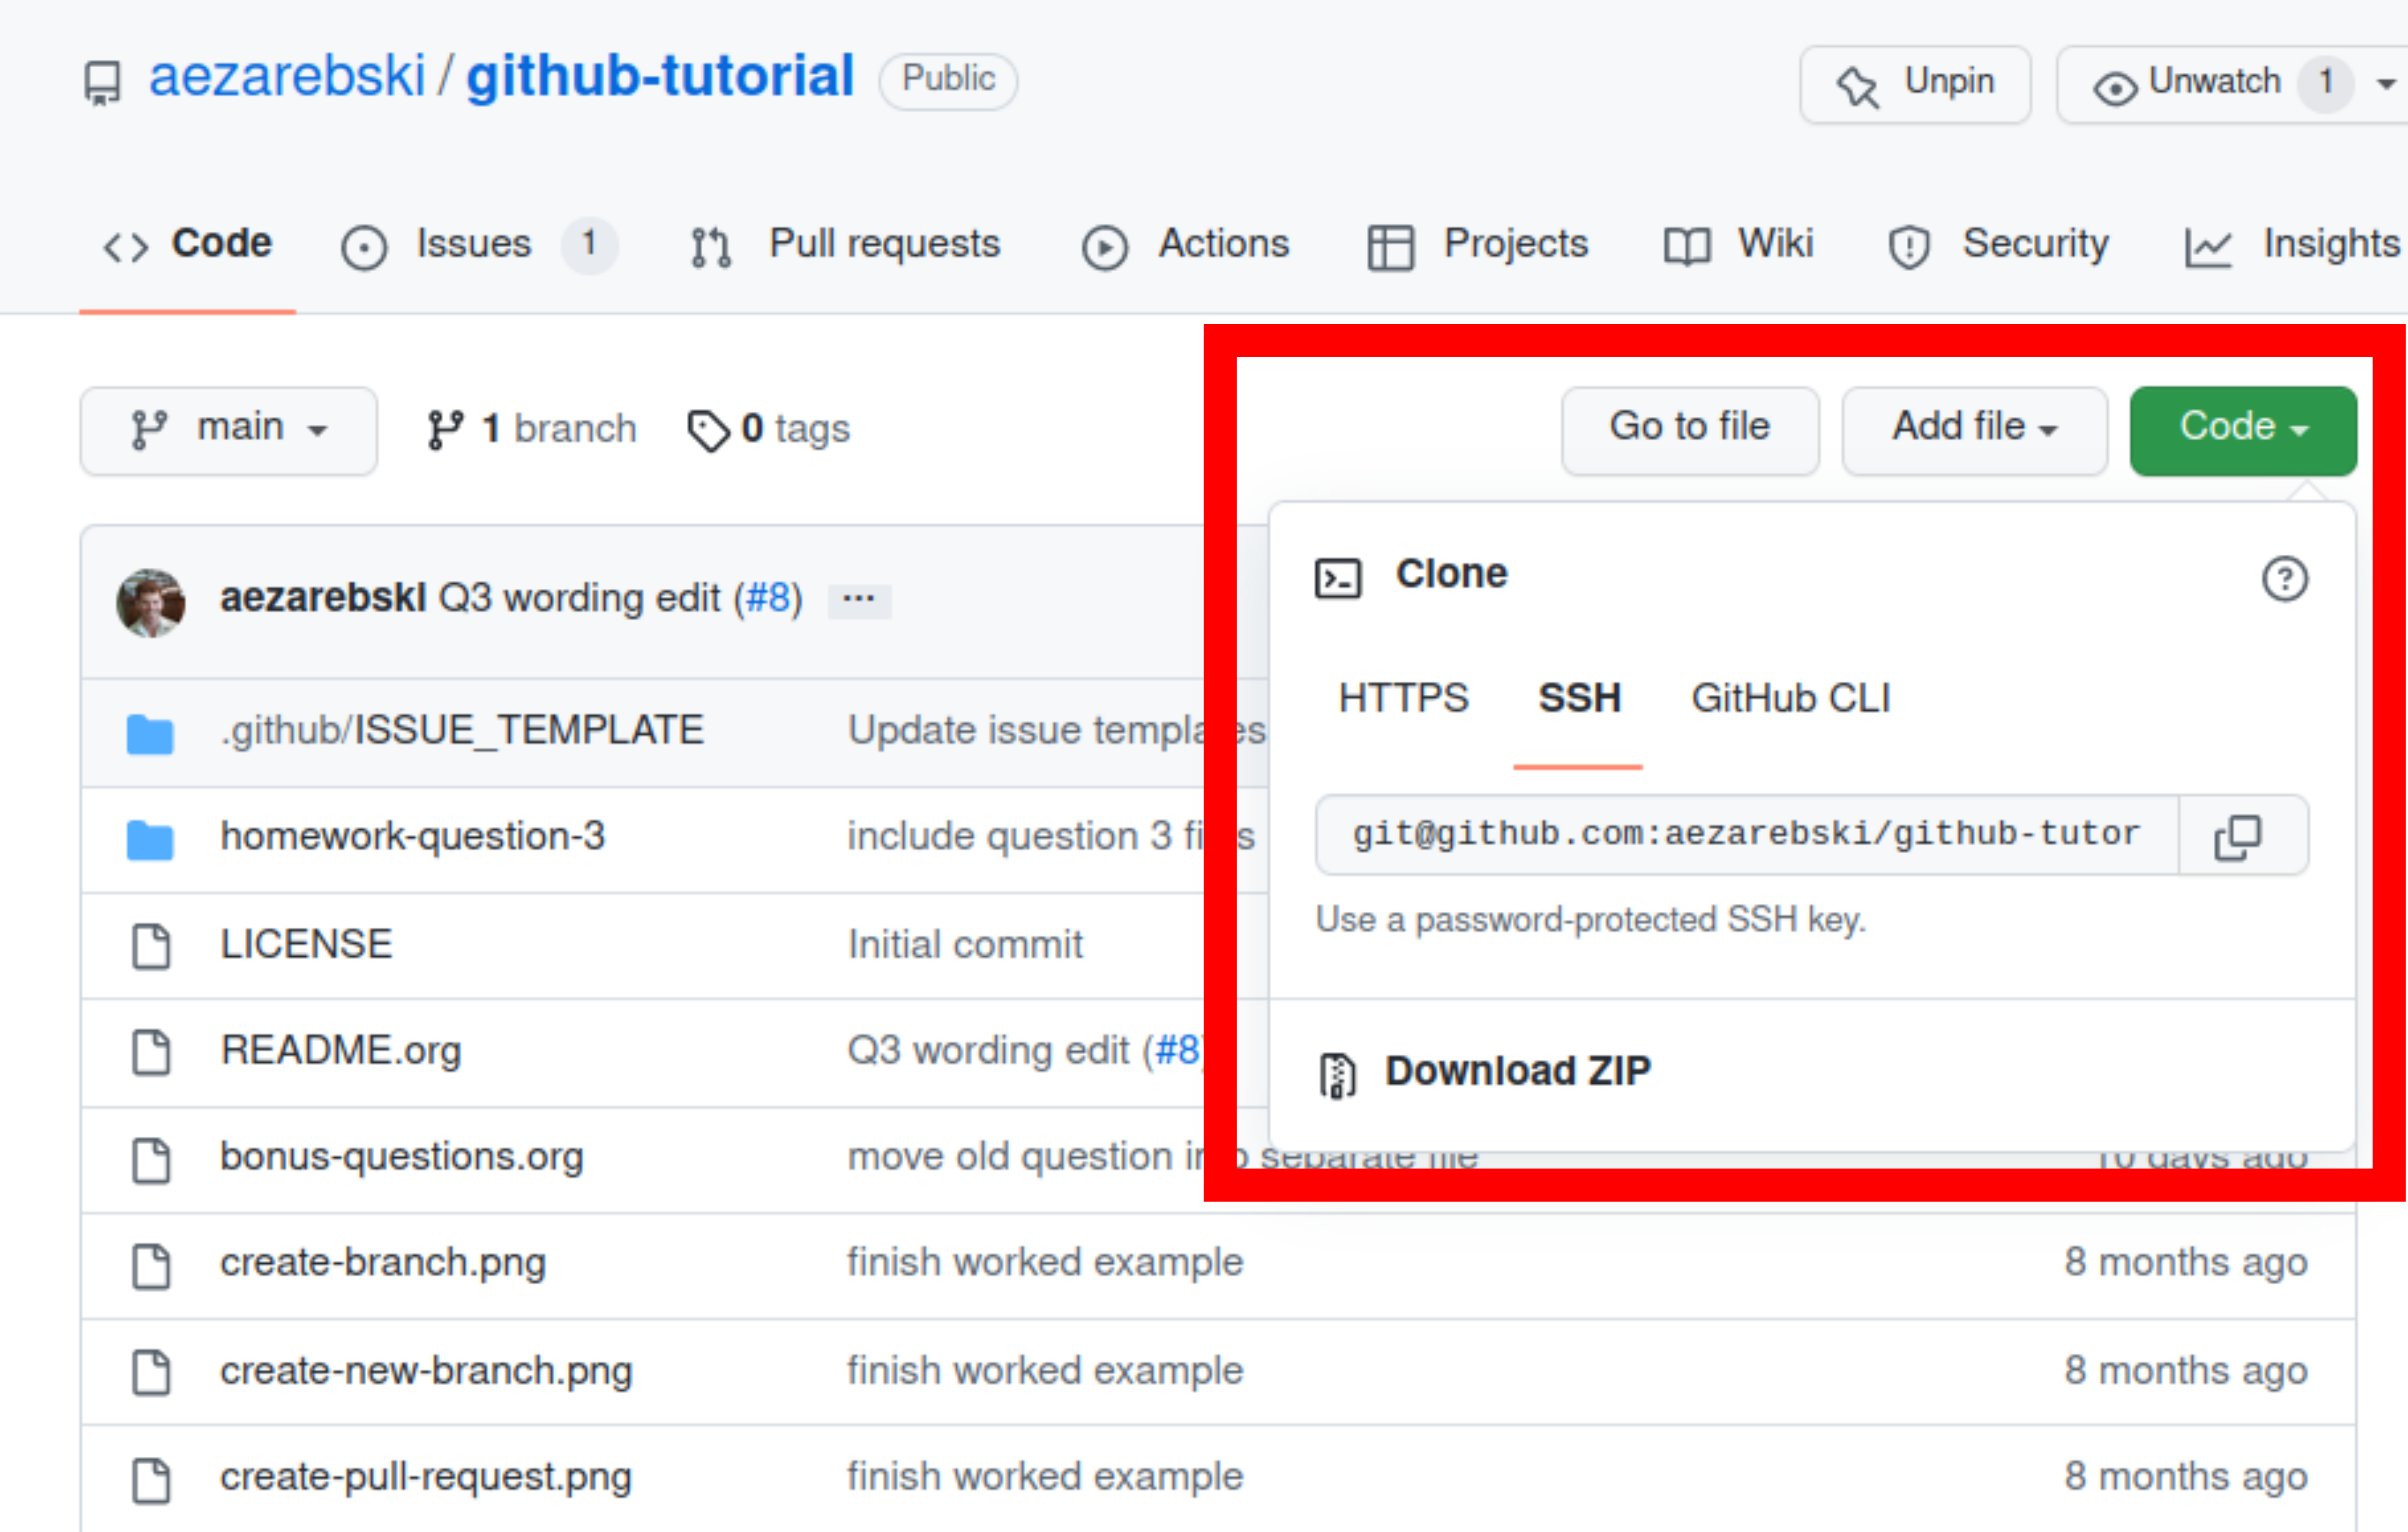
\includegraphics[width=8cm]{./download-zip-file.png}
\caption{\label{fig:download-zip-file}You can download a ZIP file containing the contents of a repository from GitHub.}
\end{figure}

\subsection{What if I am using Python, or some other language?}
\label{sec:orgdbb7313}

We have used the R programming language in this tutorial, but how we use GitHub
is language agnostic (for the most part). Most of the time, organising your data
and source code in this way is a good idea. Different programming languages
record their package versions in different ways. Recall in \hyperref[sec:org3d977e1]{this section} that we
generated a file containing the package versions. For the Python language, there
is the pip function. Running \texttt{pip freeze} at the command line will print out the
package versions. You can pipe this information to a text file (which is
conventionally called \texttt{requirements.txt}) with the following command:

\lstset{language=sh,label= ,caption= ,captionpos=b,numbers=none}
\begin{lstlisting}
pip freeze > requirements.txt
\end{lstlisting}

If you want to use multiple Python packages, it's a good idea to invest time
into learning how to set up a virtual environment. A virtual environment is an
isolated group of packages used for a project. If you want understand how to do
this, see the relevant \href{https://docs.python.org/3/tutorial/venv.html}{python documentation}.

\subsection{Upload to Zenodo}
\label{sec:org33ff0a8}

The \href{https://help.zenodo.org/}{Zenodo FAQs} contain information about how to archive a GitHub repository if
you want a more permanent form of storage. Ideally, one would archive the commit
used to generate the contents of a manuscript so it has a DOI and reference both
the archive and the \emph{live} version of the code on GitHub in the manuscript.

\subsection{Learn more about git}
\label{sec:orgb013294}

\begin{itemize}
\item \href{https://git-scm.com/book/en/v2}{Pro Git} by Scott Chacon and Ben Straub is a free book that is the ultimate
guide but is a bit technical at times.
\item \href{https://www.atlassian.com/git/tutorials}{Atlassian/Bitbucket} has excellent tutorials.
\item \href{https://learngitbranching.js.org/}{Learn Git Branching} is a game revolving around explaining git.
\item \href{https://lab.github.com/}{GitHub Learning Lab} has some introductory material on the use of git and
GitHub.
\item \href{https://stackoverflow.com/questions/tagged/git}{Stackoverflow questions} will often have answers to your questions.
\item \href{https://youtu.be/bSA91XTzeuA}{Inside the Hidden Git Folder - Computerphile} gives a bit of a behind the
scenes tour of how git works.
\end{itemize}

\subsection{Learn more about GitHub}
\label{sec:orgafdada1}

There are lots of features in GitHub that haven't been covered but may be worth
looking into:

\begin{itemize}
\item the issue tracker,
\item the wiki,
\item VSCode integration,
\item GitHub Pages\footnote{GitHub Pages offers free hosting of static websites. You may have accessed this tutorial via a GitHub Pages site.},
\item and GitHub Actions.
\end{itemize}

\subsection{Alternative solutions}
\label{sec:org7adac0d}

\subsubsection*{Git}
\label{sec:org777b0f8}

Git has the greatest market share but there are alternatives such as Subversion,
Mercurial, CVS and Darcs. Given that the overwhelming majority of people use
git, your time is probably best spent learning git. As mentioned above, if you
are going to be using git a fair bit, it is probably worth learning how to use a
\hyperref[sec:org199274b]{client} as well.

\subsubsection*{GitHub}
\label{sec:orgcc4fbea}

While git dominates the market as the choice of version control system, there
are many viable alternatives platforms to GitHub which may be more suitable for
your needs:

\begin{itemize}
\item \href{https://bitbucket.org/product/}{Bitbucket}
\item \href{https://about.gitlab.com/}{GitLab}
\item \href{https://sourceforge.net/}{SourceForge}
\end{itemize}

\subsubsection*{Zenodo}
\label{sec:orgb3e7706}

There are good general purpose alternatives to Zenodo such as \href{https://figshare.com/}{figshare} and
\href{http://datadryad.org/}{Dryad}. Institutions and journals often have a favoured provider, but they are
reasonably interchangeable. There are also numerous alternatives that are more
field specific, such as \href{http://www.gisaid.org/}{GISAID} for genomic data.

\subsubsection*{Trusting a plain text file to describe my packages}
\label{sec:org03b557c}

If you need additional assurance that your work will be reproducible, it may not
be sufficient to use \texttt{sessionInfo} (or \texttt{pip freeze} for Python) to record the
versions of the packages that you use. There are ways to capture a lot more
information about the environment you are working in so it can be recreated by
others. Unfortunately, these methods can be complex and require a lot of
configuration. Some popular examples include

\begin{itemize}
\item \href{http://rstudio.github.io/packrat/}{Packrat} which helps manage R packages,
\item \href{https://www.docker.com/}{docker} for a general purpose solution which is probably a bit overboard,
\item and \href{https://nixos.org/}{Nix} for a general purpose solution that is definitely overboard.
\end{itemize}

\section{Homework}
\label{sec:org2dd58c7}

Please ensure that in answering these questions, you use a format that is easy
to read and supports hyperlinks. The ability to include chunks of code (or
mono-spaced fonts) may be useful. You want to display the output of the \href{https://en.wikipedia.org/wiki/Tree\_(command)}{\texttt{tree}
command}. I would recommend using something like RMarkdown.

\subsection{Question 1}
\label{sec:org012eacd}

Explain (in 50--150 words) how the git, GitHub, and Zenodo complement each other
and their respective roles. Describe the value of one of the \hyperref[sec:orgafdada1]{additional features
of GitHub} not covered in this tutorial (in 50--100 words).

\subsection{Question 2}
\label{sec:org7455dc9}

Explain (in 100--150 words) the function of version control in reproducible
research. Give an example (in 50--100 words) where version control alone does
not suffice to make a piece of work reproducible.

\subsection{Question 3}
\label{sec:org5c8ce18}

This question will test your ability to organise the artefacts of a
computational project. Download the scripts and data files using the links below
and run them. Organise the files you have downloaded and the results of running
them in an appropriately structured GitHub repository. Give a brief overview of
the decisions you made along the way (in 100--200 words). Once you are happy
with this, download a ZIP file for this repository and include it as part of
your submission.

\begin{itemize}
\item \href{./homework-question-3/data-sources.txt}{Data description}
\item \href{./homework-question-3/melbourne.csv}{Melbourne rainfall data}
\item \href{./homework-question-3/oxford.txt}{Oxford rainfall data}
\item \href{./homework-question-3/combine-data.R}{First R script}
\item \href{./homework-question-3/make-plot.R}{Second R script}
\end{itemize}

If you cannot download these files directly, they should also be available \href{https://github.com/aezarebski/github-tutorial/tree/main/homework-question-3}{here}.

\subsection{Question 4}
\label{sec:orgbf11578}

This \href{https://github.com/aezarebski/biology-github-tutorial}{repository} contains an attempt at visualising two datasets. Unfortunately,
a bug was introduced somewhere during that attempt. The attempt consisted of the
following steps:

\begin{enumerate}
\item Plotting the data in \texttt{iris.csv} using \texttt{make-fig-a.R}.
\item Plotting the data in \texttt{mtcars-renamed.csv} using \texttt{make-fig-b.R}
\item Realising that there is duplicated code and refactoring it:
\texttt{reshape-data-function.R}.
\item Tweaking the figures to make them clearer.
\item And finally, realising that something is wrong with \texttt{fig-a.png}!
\end{enumerate}

Referring to the \href{https://github.com/aezarebski/biology-github-tutorial/commits/main}{commit history} of the repository, answer the following
questions (in 150--250 words \textbf{total}):

\begin{enumerate}
\item What bug was introduced, and how would you fix it?
\item How did you find the bug? How would you do this if the bug was subtle and
there were hundreds of files and thousands of commits?
\item Could you have prevented this bug by doing something differently?
\end{enumerate}

\subsection{Question 5}
\label{sec:org2ae8d28}

Read the editorial \href{https://doi.org/10.1371/journal.pcbi.1003285}{Ten Simple Rules for Reproducible Computational Research} and
(in 150--250 words \textbf{total}) give a brief explanation of how git and GitHub would
or would not be relevant to each rule.
\end{document}